
\chapter{Applications SDN et leurs apports aux data centres}

Ce chapitre définira SDN et présentera les réponses aux problématiques réseau rencontrées en général dans les data centres et qui ont été débattues dans le chapitre précédent. %Comment SDN approche la problématique ? Qu'est-ce que SDN ?
%Le chapitre démontrera également les apports de SDN au sein des data centres par rapport à ces problématiques présentées précédemment.

\section{Définition de SDN}

Les pré-requis réseaux des applications devraient être articulés dans un langage simple, utilisé pour demander les comportements réseau souhaités. La  programmation des réseaux est aujourd'hui très limitée, introduisant un malheureux compromis : obligation de développer les applications par un paramétrage réseau excessivement détaillé, ou ignorer de ces détails par le traitement du réseau comme une boîte noire.
%le développement d'applications contraint par un paramétrage réseau excessivement détaillé, ou l'ignorance de ces détails par le traitement du réseau comme une boîte noire. 
Aucune de ces solutions n'est convenable ; la première implique des applications spécifiques à chaque type de réseau alors que dans la deuxième, le contrôle nécessaire %à l'extraction de fonctionnalités réseau 
n'est pas présent. 
%The definition of network services must be application-centric and simple. The networking requirements of applications should be articulated in an IT-friendly language and used to request desired network behaviors. Today there is limited programmability, resulting in an unfortunate tradeoff. Engineering of cloud applications is either encumbered by detailed network-specific parameters and information, or ignores them and treats the network as a “black box”. Neither is optimal. The first option leads to custom applications for each network type while with the second, applications lack the visibility and control needed to leverage the true capabilities of the network.

Un niveau approprié  d'abstraction des capacités réseaux est nécessaire pour les rendre programmables et améliorer l'utilisation des ressources. L’instanciation de services réseau doit pouvoir se faire instantanément, de manière alignée aux besoins des applications. Le réseau doit permettre l'établissement de connectivité interne et entre data centres, tout en gardant la cohérence avec les politiques (de sécurité, de disponibilité et de règlementation) définies par le prestataire cloud et ses tenants. Aujourd'hui, tout cela se fait lentement, manuellement avec un risque élevé d'erreurs, comptant sur les ordres de travail pour établir une  multitude  de configurations selon le fournisseur de chaque équipement.
%The proper abstraction of network capabilities, consistent with Software Defined Networking (SDN) principles, drives programmability of network services and increases the consumability of network resources. The instantiation of network services must be instantaneous, aligned with the needs of applications. The network should act reflexively to establish the required connectivity within and across datacenters, and do so in a manner that is consistent with the defined policies of CSPs and their tenants. Today that process is slow, manual and error-prone, relying on work orders to establish a multitude of vendor- dependent configurations.

Les principes \gls{sdn} %sont plus adaptés à ce scénario, l'approche propose 
proposent une couche d'abstraction pour permettre la programmation du réseau et autoriser le contrôle dynamique de services. SDN est un nouveau \gls{paradigme} réseau défini comme une architecture qui a pour but de centraliser  sur un contrôleur l'intelligence du réseau. Cette intelligence étant traditionnellement distribuée parmi plusieurs équipements réseaux réalisant une fonction spécifique dans l'infrastructure.

Ces dispositifs ont en général une fonctionnalité de commutation de paquets (\gls{dataplane}) et une partie de traitement des données en appliquant une logique spécifique selon les états et la configuration enregistrés (\gls{controlplane}). SDN propose de dissocier ces deux fonctions dans les dispositifs et d'agréger dans un contrôleur commun l'activité de traitement. L'image ci-dessous permet de visualiser les différences entre les architectures traditionnelle et SDN. \\


\begin{figure}[h]
\begin{center}
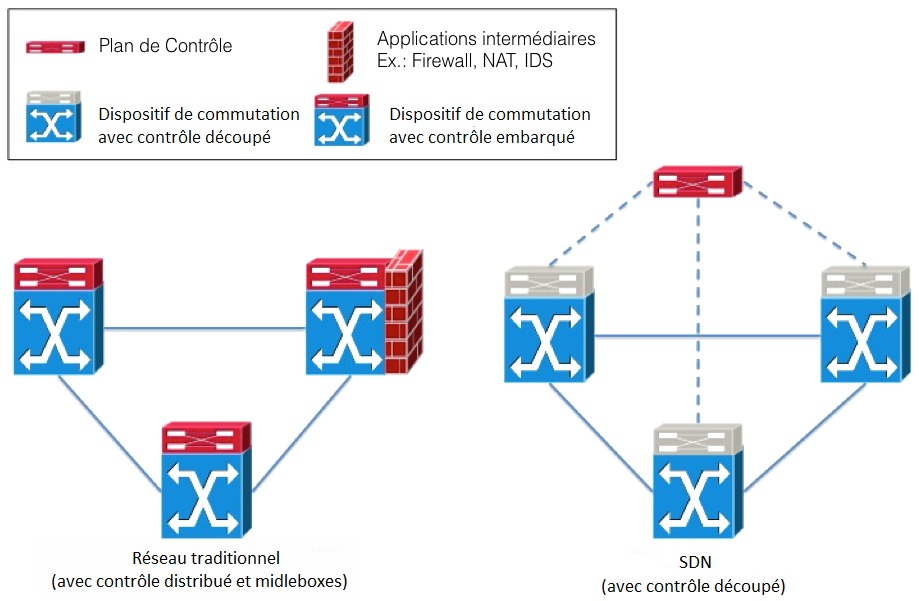
\includegraphics[width=0.7\textwidth]{images/TraditionalVsSDN} 
\caption{Architectures : réseau traditionnel et SDN. \cite{SurveySDNArchi}} \label{TraditionalVsSDN}
\end{center}
\end{figure}


L'expérience, lors de la construction des grands réseaux IP/MPLS, a montré que l'intelligence doit être poussée vers la périphérie pour autoriser l'extension des réseaux. Le principe doit être appliqué afin de promouvoir un cœur du réseau data centre simplifié et efficace. L'approche sépare les services réseaux de l'infrastructure physique permettant l'innovation parallèle dans les deux domaines.

%Application of lessons learned from building very large IP/MPLS networks. In the “thin waist” model for scaling IP networks, intelligence is pushed to the edges. The same is in order for promoting a simple and cost-effective core datacenter network, consistent with the manner in which IP technologies have successfully scaled to date. The approach decouples network services from the infrastructure and enables parallel innovation in each domain.

Les leçons acquises lors de la conception des réseaux mobiles ont apporté la technique d'optimisation pour la mobilité et d'automatisation opérationnelle à large échelle. Cela permet la création d'un modèle auto-instancié et dirigé selon les règles établies qui minimise les coûts d'implémentation et délais de livraison de service.
%Application of lessons learned from design of mobile networks that have been optimized to provide mobility and operational automation at massive subscriber scale. This yields a policy-driven auto-instantiation model for the datacenter network that minimizes costs and delays. The new model significantly changes the game, greatly increasing the efficiency with which cloud services canbe delivered.

%En complément de ces principes, SDN propose également une interface commune de programmation du réseau sous-jacent, grâce à l'abstraction de ses capacités.
%Bringing common IT language to programming the underlying network by abstracting the network capabilities into IT and business logic terminology.

Cette solution apporte comme bénéfice l'introduction d'une interface commune et programmable de management, permettant la mise en place dynamique de services, indépendamment de la marque/modèle des dispositifs réseau. Avec SDN, l'administration réseau devient plus agile car un seul élément (le contrôleur) est à maîtriser au lieu d'avoir à configurer l'ensemble des équipements du système, ce qui accélère considérablement le temps de convergence du réseau pour l'accommodation de nouvelles applications déployées. \cite{SDNNewNormONFExecutiveSummary} \cite{ImplementationChallengesForSDNBackground}





\section{Virtualisation des fonctions réseau, NFV}


Un concept qui est très souvent discuté en parallèle à \gls{sdn} est \gls{nfv}. \gls{nfv} pousse les technologies de virtualisation à consolider les applications réseau sur des serveurs, switches et baies de stockage standard de l'industrie. La virtualisation des fonctions réseau non seulement réduit les dépenses en équipements, mais aussi apporte d'autres bénéfices tels que l'extension agile d'applications, à une vitesse plus rapide, une plus haute disponibilité et une meilleure utilisation de ressources.
%A concept that often gets discussed in conjunction with SDN is Network Function Virtualization (NFV).
%NFV leverages standard virtualization technologies to consolidate network applications – which have traditionally been hosted on proprietary hardware appliances – onto industry standard servers, switches and storage. In addition to reducing expenditure on equipment costs, virtualizing network functions also brings benefits such as rapid scaling of applications, faster speed of innovation, increased high availability and improved resource utilization. 

Toutefois, pour bénéficier de ces apports, il est nécessaire que l'infrastructure réseau sous-jacente s'adapte rapidement et automatiquement. Par exemple, pour migrer une fonction réseau  dans un nouveau matériel, les politiques et les configurations associées à ce service doivent être provisionnées dans beaucoup d'autres équipements et fonctions. La complexité à configurer les réseaux dans un environnement si dynamique augmente énormément avec l'introduction de nouveaux éléments réseaux.
%However, realizing these benefits requires that the underlying network infrastructure is adapted quickly and automatically. For example, for a network function to either scale up or migrate onto a new piece of hardware, the security and policy configuration associated with that network function may have to be provisioned on a large number of switches and other network functions. The complexity of configuring networks in such a dynamic environment increases greatly as the number of network elements increase.


Bien que les développements de SDN et NFV puisse progresser indépendamment, l'association des deux principes est d'un fort intérêt pour le progrès des solutions cloud. SDN peut être employé en tant que technologie facilitatrice de la virtualisation des fonctions réseau, favorisant la consolidation des applications réseau dans des dispositifs industriels standard. \cite{OFSDNNFVintro} \cite{realTimeCloudNFV} \cite{IntelCloudEPC}

%Mainstream industry adoption and deployment of Cloud Telecoms will be hindered, or even blocked, until carrier grade telecom requirements have been fully proven on the key technologies underpinning the Cloud Telecoms concept, namely Network Functions Virtualisation (NFV), Software Defined Networking (SDN) and deployment on industry-standard, high- volume servers.
%While the development of SDN and the development of NFV can proceed independently, there are some areas of possible overlap and cooperation.

%When services are needed, these components are assembled (or orchestrated) and deployed on servers. The NFV plan is to support everything from bare metal to an architected cloud as a hosting platform. Once deployed, they are managed so as to create as good of a service experience as the original devices would have created.



\section{SDN, NFV et le Cloud Computing}

Les approches Cloud permettent aux opérateurs réseau d'assurer une création et un déploiement de services plus rapides. Elles répondent également aux attentes croissantes sur la qualité et la performance des solutions, tout en traitant les charges trafics de plus en plus importantes.


%Cloud-based approaches enable network operators to ensure rapid service creation and rollout by delivering new levels of flexibility, scalability and responsiveness. They also satisfy the growing expectations for service performance and QoE, while handling ever-increasing traffic loads.Operators are making use of NFV, SDN and cloud technology in three ways:
%> Telecom cloud – operators are gradually turning their networks into layered and distributed clouds, in which workloads can be located to optimize QoE or data transport, and to offer the best possible elasticity.
%> IT cloud – operators are optimizing the use of internal IT resources to deliver an improved customer experience, to accelerate time to market for innovative and compelling services, and to improve their efficiency for cost reduction.
%> Customer cloud – operators leverage a platform, or their own cloud, to resell or broker value-added cloud services.
%Although these scenarios are all quite different, they share some common requirements, and operators can benefit from the implementation of a common platform across all three scenarios.

Afin de supprimer les contraintes des réseaux dans les data centres, une plateforme innovante pour l'abstraction des fonctionnalités réseau et pour l'instanciation automatisée de services est proposée. Avec SDN, les fournisseurs de services cloud, opérateurs à l'échelle web et grandes entreprises technologiques peuvent construire une infrastructure réseau multi-tenante, robuste et extensible pour délivrer des espaces virtuels de compute, stockage et réseau prêts à l'usage pour des milliers de tenants et groupes d'utilisateurs.

%Nuage NetworksTM removes the constraints of the datacenter network through an innovative Virtualized Services Platform (VSP) that abstracts network capabilities and automates service instantiation. With the Nuage Networks Software Defined Networking solution, cloud service providers, web-scale operators and large tech enterprises can b uild a robust and scalable multi-tenant networking infrastructure that delivers secure virtual slices of readily consumable compute, storage and networking instantaneously across thousands of tenants and user groups.


%Combining a Network-enabled Cloud approach (which offers flexible management of cloud applications) with NFV (several virtualized applications on a common hardware platform, which reduces opex and capex) and the real-time control capabilities of Service Provider SDN (as shown in Figure 3) yields significant advantages. 
%First, it enables operators to more easily (and usually automatically) adapt network characteristics and resources to serve the more dynamic and real-time nature of new services. 
%Second, it extends the virtual infrastructure beyond the traditional computing and storage resources to enable applications to encompass WAN resources – making it easier to engage one or more data centers, as well as any other intelligent nodes in the network.
%Network-enabled Cloud delivers the flexibility and elasticity to deploy software applications and virtualized network functions wherever they are needed in the network. This improves time to market and enhances innovation, QoE and network efficiency.

Le \gls{controlplane} dans SDN fonctionne en lien avec le système de management cloud afin de configurer dynamiquement des éléments réseaux pour s'adapter aux décisions des systèmes d'orchestration pour le changement d'utilisations des ressources. SDN fournit l'infrastructure nécessaire pour réaliser cette capacité de NFV étendue.
%The control plane in software-defined networks works in conjunction with cloud management systems in order to dynamically configure network elements to adapt to changing resource usage decisions made by cloud orchestration systems. SDN provides the infrastructure required to truly realize the potential of NFV.

La figure \ref{cloud-sdn-nfv} affiche comment SDN et NFV s'intègrent dans une infrastructure Cloud pour atteindre les objectifs de virtualisation du réseau. \\

\begin{figure}[h]
\begin{center}
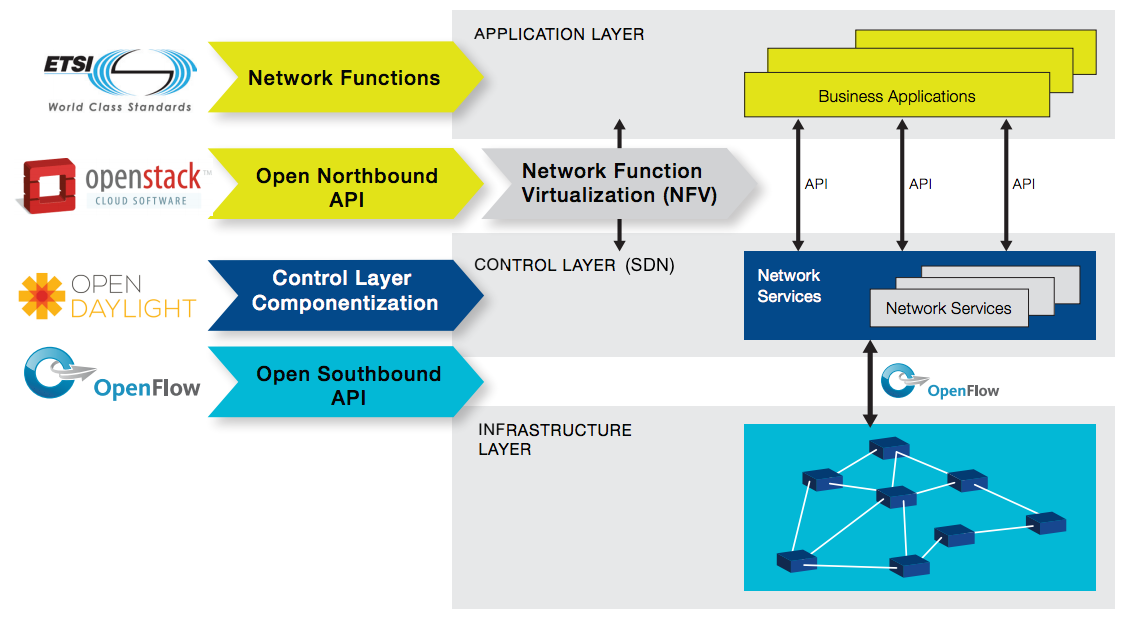
\includegraphics[width=0.8\textwidth]{images/cloud-sdn-nfv} 
\caption{SDN, NFV et Cloud Computing. \cite{OFSDNNFVand}} \label{cloud-sdn-nfv}
\end{center}
\end{figure} 

L'image montre également les protocoles et standards ouverts qui émergent pour chaque technologie comme \gls{openflow} pour la communication entre les dispositifs réseau et le contrôleur SDN (\gls{opendaylight}), \gls{openstack} pour la gestion Cloud et ETSI pour le NFV. Il est important de noter que de grands noms de l’industrie (comme Cisco, Microsoft, Google etc.) se sont engagés dans ces projets pour accélérer le développement de ces technologies.

Dans le cloud, avec SDN et NFV travaillant ensemble, on peut dynamiquement étendre les fonctions réseau au sein des data centres. Par exemple, lorsque la charge réseau augmente, le contrôleur SDN peut demander au gestionnaire cloud d'instancier une nouvelle fonction réseau dans le cloud pour redistribuer et répartir le trafic. 
%(pas claire) Another case that brings out the value of a combined real-time programmable network and cloud solution is the ability to dynamically extend network functions into the cloud – with SDN, NFV and the cloud all working together. As the load on a network appliance increases, the SDN controller can request a peer cloud manager to instantiate a virtual network function in the cloud and to start load balancing between the physical appliance and the virtual appliance, treating it as a common entity.

%However, fully realizing the potential of this technology in today’s service provider networks means doing more than just separating the forwarding and control planes. This expanded definition of Service Provider SDN includes:

%> Integrated network control – this unified control layer controls the data center and network as an integrated entity, in order to deliver the best user experience.
%> Orchestrated network and cloud management – a unified approach that includes legacy network management and new cloud management systems. It is this end-to-end orchestration that enables flexible service creation, which in turn makes the network dynamic, adaptive and agile. This cuts introduction and modification cycles for services and removes barriers to innovation.
%> Service exposure – the SDN architecture provides network awareness to the application layer through service exposure application programming interfaces (APIs). These APIs not only provide raw network data, but are instead composed APIs that deliver actionable information at the application level.

La couche de contrôle SDN apporte l'allocation de ressources extensible et en temps-réel pour les besoins des services réseaux. Cela permet que les services soient définis et provisionnés très rapidement via de portails libre services. Le service est mis à disposition dans un délai de minutes, au lieu de jours ou même semaines comme il est traditionnellement nécessaire.
%The service control layer of the Service Provider SDN architecture brings elastic, real-time allocation of resources for networking services. It enables these services to be defined and provisioned through self-service portals in a matter of minutes, rather than the days, weeks or even months that are traditionally required.

Cette plateforme, avec un contrôle intégré à travers des domaines réseaux, expose des \glspl{api} qui permettent aux applications d'instancier dynamiquement des ressources pour accomplir ces objectifs métiers. Un  système de management de l'infrastructure fournit des capacités supplémentaires, comme une planification plus fiable, approvisionnement, activation, adaptation et le contrôle de nouvelles connexions de services.
%This demands a platform with integrated control across networking domains that exposes “composed APIs” for new revenue generation. An end-to-end network management system across IP and transport infrastructure provides further efficiencies, develops greater responsiveness, and enables more reliable planning, provisioning, activation, adaptation and control of new service connections.

SDN permet de coupler la gestion du cloud au réseau programmable, achevant une intégration complète du réseau. Avec une orchestration commune des services, on obtient une réduction des coûts opérationnels pour l'approvisionnement et la supervision ainsi qu'une création flexible de services. Cela rend le réseau dynamique, adaptatif et agile, donc prêt pour le Cloud. \cite{OFSDNNFVand} \cite{realTimeCloudNetworkEnabled} 
%The goal is to couple cloud management to a programmable network, via SDN controllers, to achieve full integration of the cloud and network, where cloud resources are no longer confined to a single data center, but are spread throughout the network.

%Using common orchestration for end-to-end service management as well as for operations, administration and maintenance reduces operating costs in areas such as provisioning, monitoring and faultfinding. More importantly, end-to-end orchestration enables flexible service creation, which makes the network dynamic, adaptive and agile.
